\documentclass[11pt]{article}
\usepackage[letterpaper,margin=1in]{geometry}
\usepackage[T1]{fontenc}
\usepackage{microtype}
\usepackage[hidelinks]{hyperref}
\usepackage{fancyhdr}
\usepackage{enumitem}
\usepackage{tikz}
\setlength{\parindent}{0pt}
\setlength{\parskip}{0.62em}
\emergencystretch=2em
\pagestyle{fancy}
\fancyhf{}
\fancyhead[L]{\small The Open System Has a Body}
\fancyhead[R]{\small Working Paper}
\fancyfoot[C]{\thepage}
\begin{document}
% CHECKPOINT: SCF-20260817-BMC-003
% SCHEMA: ANCIENT MASTER / SLIPCASE v15.5-AM
% RETURN: 000__RETURN_PATH.txt

\begin{titlepage}
\thispagestyle{empty}
\vspace*{0.7in}
{\huge\bfseries The Open System Has a Body\par}
\vspace{0.12in}
{\Large Hidden Infrastructure, Task Change, and the Limits of Self-Organization\par}
\vspace{0.5in}
{\large Watson Hartsoe\par}
\vspace{0.2in}
{\small WORKING PAPER\par}
\vfill
{\small SCF-20260817-BMC-003 · 17 August 2026 · 23 cards\par}
\end{titlepage}

\begin{abstract}
Experimental organizations often describe openness by subtraction: fewer grades, fewer leaders, fewer prescribed agendas, fewer constraints. Across Black Mountain College, Black Mountain SOLE, Sugata Mitra's SOLE design, Harrison Owen's Open Space Technology, Jo Freeman's account of structurelessness, and the Granny Cloud's own history, a different mechanism appears. Self-organization repeatedly depends on conditions that vanish from view when they work: device ratios, facilitator timing, volunteer attention, physical access, connectivity, boundary translation, and task-specific coordination. Two failures are especially diagnostic. First, Black Mountain SOLE's showcase success bypassed the MOOCs that nominally defined the experiment. Second, the Granny Cloud's online relation became unavailable when children could not reach physical centres and volunteers themselves aged. These cases suggest that the relevant unit is neither structure nor freedom but the placement, task-fit, infrastructural support, and revisability of constraints. I develop ``structured openness'' as a provisional hypothesis and propose a constraint ledger for testing it rather than treating it as a celebratory label.
\end{abstract}

\textbf{Keywords:} self-organization; experimental education; infrastructure; organizational structure; Black Mountain College; open systems; pedagogy

\textit{Evidence note.} Source-grounded claims are cited. ``Structured openness,'' the constraint ledger, and connective synthesis are compiler-derived from the preserved card field. They are hypotheses, not terminology attributed to the cited authors.

\section{The wrong variable: amount of structure}
Carl DiSalvo's account of Black Mountain College begins from an institution that was visibly unstable but not simply careless. The college omitted several devices associated with ordinary institutional stability, yet DiSalvo also emphasizes the labor required to maintain the experiment and calls it ``methodical'' rather than efficient \cite{disalvo2026blackmountainmess}. This distinction matters because it breaks the easy opposition between order and mess. If an institution can be methodical while leaving many outcomes unsettled, the relevant question is not whether structure exists. It is where structure has been placed.

The shadow transcript makes the point concrete. Black Mountain could reject grades as a governing educational representation while preserving grades as a translation device for students who needed conventional transcripts elsewhere \cite{disalvo2026blackmountainmess}. A representation may be refused internally and retained at the boundary. The institution's openness therefore depended partly on machinery that did not announce itself as the centre of the educational philosophy.

Harrison Owen's Open Space Technology pushes this relocation further. Open Space famously begins with a blank agenda, but Owen's guide does not describe an undefined environment. It specifies a compelling theme, interested and committed participants, a time, a place, a leader, an agenda-generation procedure, and a mobility rule \cite{owen_open_space_guide}. The blank wall is an output of prior specification. What remains open is the trajectory participants generate inside a bounded container.

This yields a first proposition: productive openness is not structurelessness but \emph{selective formalization}. The arrangement fixes some variables so that others can remain unresolved. That statement alone, however, is too weak. Every organized activity has conditions. To become useful, the analysis has to ask which conditions, for what task, sustained by what infrastructure, and revisable by whom.

\section{Designed scarcity and the return of the teacher}
Sugata Mitra's SOLE Toolkit makes the material design of self-organization unusually visible. The toolkit specifies group movement, sharing, large questions, investigation, review, and a deliberately limited number of computers. It recommends roughly one computer per four learners and presents that scarcity as a means of producing peer interaction \cite{mitra_sole_toolkit}. Too few devices are not treated as an implementation defect. Scarcity is used as a social operator.

That design should not be romanticized. A bottleneck can produce collaboration, but it can also produce domination by the confident keyboard user, spectatorship, waiting, or exclusion. The card field therefore treats device scarcity as a testable mechanism rather than a virtue. The point is narrower: what looks like freedom at the level of curriculum may be generated by highly specific constraints at the level of material arrangement.

The same migration occurs with teaching. SOLE rhetoric decentralizes answer-giving, yet the toolkit retains adult encouragement and remote mediators. The ``Skype Granny'' is not primarily an answer source; she can support language, search, confidence, attention, and persistence \cite{mitra_sole_toolkit}. Removing authoritative content delivery does not remove pedagogical labor. It redistributes that labor into affective and infrastructural functions that are easier to mistake for atmosphere.

This is where the notion of hidden constitutional layer begins to sharpen. A learner may be free to determine what she finds, but her capacity to remain in the search depends on an environment already populated by devices, questions, social ratios, adults, schedules, and review practices. The trajectory is open because the conditions are not.

\section{A form can work until the task changes}
Jo Freeman's ``The Tyranny of Structurelessness'' supplies a missing temporal variable. Her argument is often reduced to the slogan that structurelessness conceals hierarchy. The more useful mechanism here is task change. Freeman describes loose, informal groups as well suited to consciousness-raising, then shows how problems emerge when groups move toward more specific coordinated work without changing the form through which they coordinate \cite{freeman1972tyranny}.

This reframes a large part of the Black Mountain/SOLE problem. An organizational form can be successful evidence for itself under task T1 and become disabling under task T2. A meeting protocol can generate an agenda beautifully in a bounded event and become ambiguous when treated as a general philosophy of schooling. A peer network can support exploration and become inadequate when scholarships, housing, budgets, or institutional survival require consequential allocations. The relevant variable is not ``more structure'' but fit between current task and coordination form.

Freeman also distinguishes formal and informal structure. Making formal rules explicit does not abolish informal relations, but it can make authority visible enough to challenge \cite{freeman1972tyranny}. This matters for experimental institutions that describe themselves as horizontal. If the rules of consequential decision-making remain tacit while material power remains concentrated, the rhetoric of openness can make actual power harder rather than easier to inspect.

The comparison is conceptual, not genealogical. There is no evidence in this checkpoint that Black Mountain SOLE, Owen, Mitra, or historical Black Mountain College drew on Freeman. The value of the comparison is discriminating: it suggests that protocol migration should be tested against task migration. A technique adequate to one task cannot be assumed adequate to another because both are described as participatory.

\section{The stepping stone that bypassed the theory}
Black Mountain SOLE offers an accidental ablation test. Nora Caplan-Bricker reports that Chris Coleman became the institution's first major case study after his startup won seed funding, yet he had taken no MOOC \cite{caplanbricker2013blackmountain}. This does not prove that MOOCs were useless to other participants. It does show that the component used to describe the experiment was not necessary for a showcase success.

The useful response is not to rescue the original theory but to move outward. What did the successful participant actually use? Residential time, peers, entrepreneurial language, mentors, introductions, legitimacy, project focus, or simply freedom from another schedule? The current evidence cannot answer. The failure of the nominal component nevertheless changes the target of inquiry. When the advertised technology can be removed and the valued outcome remains, the surrounding field becomes the research object.

This ``success-by-bypass'' is more informative than a conventional success story because it separates description from mechanism. The experiment may have built something other than what it thought it built. That possibility recurs throughout the deck: grades remain as shadow infrastructure after their educational authority is rejected; startup metrics enter an anti-credential environment; expert pedagogy returns as encouragement; a blank agenda is generated by a facilitator-protected boot sequence. The apparently incidental machinery repeatedly becomes causal.

\section{The cloud had bodies}
The Granny Cloud history pushes this insight beneath the interface. The project's official account describes remote volunteers connecting with children through online conversations, but its historical interruptions reveal the physical conditions on which that relation depended. Early centres closed in part because of funding constraints and school apathy. During COVID-19, many children could no longer reach the centres from which they connected and often had minimal or no home internet. The organization also names ageing volunteers and health challenges in explaining its 2022 wind-down; in 2026 it reports restarting at one location with a fresh volunteer team \cite{grannycloud_background}.

The point is not that an online system secretly occurs offline. The stronger claim is operational: the availability of the relation depends on bodies and sites at both ends. A ``cloud'' of encouragement can disappear locally because a child cannot reach a terminal, a home lacks connectivity, a coordinator cannot sustain a centre, or volunteers age out of the labor that keeps the relation alive.

This changes what counts as infrastructure in theories of self-organized learning. If encouragement, language support, continuity, and search persistence are part of the pedagogical mechanism, then the bodies supplying them cannot be treated as incidental to a digital model. Likewise, if children need shared centres to access the system, then spatial access is part of the computationally mediated environment. The cloud is not merely content delivered over a network. It is a maintained relation among places, devices, connectivity, schedules, institutions, and people.

The source is the Granny Cloud's own organizational history, so its causal account should not be treated as an independent evaluation. Funding, local coordination, design choices, and school participation may matter alongside the factors it names. That limitation is productive: it turns ``the cloud had bodies'' into a test rather than a slogan. A stronger study would reconstruct centre-level timelines and ask which combinations of access, connectivity, volunteer availability, funding, and coordination predict continuity.

\section{Voice, complaint, and constitutional contestability}
Once specification is relocated into conditions, the political question is who can alter those conditions. Caplan-Bricker's Black Mountain SOLE reporting distinguishes conversational horizontality from control over scholarships, housing continuity, and institutional resources \cite{caplanbricker2013blackmountain}. Everyone may have a say while only some actors can execute the state transition that determines whether another participant can remain.

Open Space contains a parallel problem in procedural form. Its Law of Two Feet assigns participants responsibility for moving where they can contribute; its agenda-generation procedure makes participants responsible for proposing what they care about \cite{owen_open_space_guide}. Inside a short, voluntary event this can be an effective agency mechanism. Transplanted into an institution with unequal money, expertise, time, or vulnerability, the same operation can translate missing support into personal responsibility: invent the missing teacher, create the absent program, move elsewhere, or accept that the issue was not raised.

The distinction is between freedom \emph{inside} a protocol and authority \emph{over} the protocol. Owen's guide itself retains facilitator control over the transition that bootstraps the agenda. Freeman's analysis supplies the corresponding governance warning: when rules remain informal, power can remain legible only to insiders \cite{freeman1972tyranny}. The problem is therefore not that a constitutional layer exists. The problem is that an ideology of structurelessness or horizontality can make it difficult to identify, challenge, or revise.

This yields a stronger criterion than ``openness.'' Productive openness requires \emph{constitutional contestability}: participants need some intelligible way to distinguish a failure inside the experiment from a failure of the apparatus that structures the experiment, and some path by which evidence can reach that apparatus.

\section{Structured openness as a testable wager}
The previous checkpoint contained \texttt{[[Structured Openness]]} as an unresolved address. In this run the address is provisionally occupied by a new card, but the move is deliberately reversible. The concept is useful only if it makes different predictions than the generic statement that all systems have structure.

A compact representation is a four-part constraint ledger:

\begin{description}[leftmargin=1.1in]
\item[T] the current task or problem field;
\item[C] conditions held comparatively fixed;
\item[X] participant-generated trajectories left open;
\item[A] the authority or process by which the fixed conditions can be inspected and revised.
\end{description}

Structured openness can then be defined provisionally as an arrangement in which X remains substantively underdetermined while C is sufficiently specified to make participation possible, C remains fitted to T, and A allows learning to reach the layer that structures the experiment. The definition exposes several failure modes.

First, if C is invisible, existing expertise or informal networks can become a hidden curriculum. Second, if C is inaccessible, participants may be free inside the system while unable to challenge the system's conditions. Third, if T changes while C remains fixed, structural lag appears. Fourth, if the infrastructure supporting C fails, nominal freedom becomes unusable. Fifth, if X is over-specified, openness collapses into ordinary prescription. Sixth, if C is under-specified relative to participants' capacities, openness can be experienced as drift or abandonment.

This framework integrates the field without pretending its cases are equivalent. Historical Black Mountain College supplies the distinction between method and efficiency and the persistence of boundary translation \cite{disalvo2026blackmountainmess}. Mitra supplies deliberately engineered social/material conditions \cite{mitra_sole_toolkit}. Owen supplies a bounded protocol whose open agenda depends on a prior frame \cite{owen_open_space_guide}. Freeman supplies task-relative structure and contestable formalization \cite{freeman1972tyranny}. Black Mountain SOLE supplies hidden curriculum, resource asymmetry, and success-by-bypass \cite{caplanbricker2013blackmountain}. The Granny Cloud supplies infrastructural interruption at the level of places, connectivity, and bodies \cite{grannycloud_background}.

The test is severe by design. Build the ledger for each institution and for different periods within each institution. If T, C, X, and A cannot distinguish successful from failed arrangements, generate new predictions, or identify different intervention points, then ``structured openness'' should be discarded. The concept is not saved by sounding right.

\section{Limits and unresolved territory}
This checkpoint remains small and uneven. The historical Black Mountain argument depends heavily on a contemporary essay drawing on Martin Duberman rather than on direct archival coding. The proposed Open Space-to-SOLE genealogy remains unproven: textual correspondence motivates a search but is not evidence of transmission. The SOLE device-ratio card derives from the toolkit's design rationale, not from observational evidence about keyboard control, talk distribution, or learning outcomes. The Granny Cloud source is an organizational self-history. Freeman's essay is used comparatively rather than genealogically.

These limits point directly toward the next work. The most important empirical move is to build constraint ledgers from primary records rather than from retrospective descriptions. For historical Black Mountain College, that means identifying which stabilizers were deliberately refused, which were financially unavailable, and which persisted informally. For Black Mountain SOLE, it means reconstructing decision rights and resource control rather than accepting claims of horizontality. For Open Space, it means separating local exit within a bounded event from exit from the institutional container. For SOLE and Granny Cloud, it means tracing access, device control, mediator labor, and continuity at the level where participants actually encountered the system.

The open field is therefore not a weakness of the argument. It is the mechanism by which the argument remains falsifiable.

\section{Conclusion}
The strongest finding in this research field is not that open systems need structure. That claim is too general to matter. The stronger proposition is that openness is produced by a particular placement of constraint, and that the consequences of those constraints depend on task, infrastructure, and revisability.

The blank wall has a frame. The shared computer has a ratio. The encouraging mediator has a body and a schedule. The supposedly irrelevant transcript keeps an external boundary traversable. The structureless group has informal decision rules. The showcase success can bypass the technology used to describe the experiment. These are not exceptions surrounding an otherwise pure form of self-organization. They are evidence about where the program actually lives.

Structured openness is the name proposed here for a research problem: how to leave substantive trajectories unresolved while making the conditions that enable them visible enough to maintain, test, and revise. Its opposite is not structure. Its failure is a field in which the conditions governing participation become hidden, mismatched to the task, infrastructurally unusable, or unreachable by criticism.

The next step is not to believe the concept harder. It is to run the ledger and see whether the cases force it to become more precise—or make it disappear.

\begin{thebibliography}{9}
\bibitem{disalvo2026blackmountainmess} Carl DiSalvo. ``Black Mountain College Was a Mess.'' \emph{Under The Circumstances}, 12 August 2026. \url{https://underthecircumstances.substack.com/p/black-mountain-college-was-a-mess}.
\bibitem{caplanbricker2013blackmountain} Nora Caplan-Bricker. ``This North Carolina Campus Was Meant to Show Off the Future of Online Education.'' \emph{The New Republic}, 22 December 2013. \url{https://newrepublic.com/article/116014/black-mountain-sole-mooc-campus-online-learners-has-rough-start}.
\bibitem{mitra_sole_toolkit} Sugata Mitra. \emph{SOLE Toolkit: How to Bring Self-Organised Learning Environments to Your Community}. School in the Cloud, n.d. \url{https://motricidadehumana.org/wp-content/uploads/2015/11/sole_toolkit_web_2-6.pdf}.
\bibitem{owen_open_space_guide} Harrison Owen. ``A Brief User's Guide to Open Space Technology.'' Open Space World, n.d. \url{https://openspaceworld.org/wp2/hho/papers/brief-users-guide-open-space-technology/}.
\bibitem{freeman1972tyranny} Jo Freeman. ``The Tyranny of Structurelessness.'' \emph{The Second Wave} 2(1), 1972. Author text: \url{https://www.jofreeman.com/joreen/tyranny.htm}.
\bibitem{grannycloud_background} The Granny Cloud. ``Background \& History.'' n.d. \url{https://thegrannycloud.org/about/background/}.
\end{thebibliography}

\section*{Appendix: Assembly Instrument}
This working paper was assembled from the SLIPCASE research field under checkpoint SCF-20260817-BMC-003. The exact compilation instrument is preserved at \nolinkurl{_PROMPTS/ANCIENT_MASTER_SLIPCASE_v15.5-AM.xml}. Its SHA-256 is\\ \nolinkurl{722788a5e436665054eb7d8dfadcaa81c96f05fe693f46ce59e71129dd79351f}. The prompt is methodological provenance, not evidence for the paper's claims. Rebuild instructions are in \nolinkurl{000__REBUILD.txt}.

\section*{Colophon}
This paper is derived and regenerable. Archived zettel payloads and preserved source materials remain distinct from the argument above. Production history: \nolinkurl{the-open-system-has-a-body__MAKING_HISTORY.txt}. Return path: \nolinkurl{000__RETURN_PATH.txt}.

\begin{flushright}
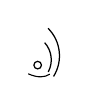
\begin{tikzpicture}[scale=.48,baseline=-1pt]
\draw[line width=.45pt] (0,0) circle (.10);
\draw[line width=.45pt] (.28,-.18) arc (-28:42:.68);
\draw[line width=.45pt] (.42,-.30) arc (-32:45:1.03);
\draw[line width=.40pt] (-.25,-.23) .. controls (0,-.34) and (.18,-.33) .. (.32,-.24);
\end{tikzpicture}
\end{flushright}
\end{document}
